\section{Classification}

Classification is a supervised learning task where the goal is to assign input $x$ to discrete labels $y$. Examples include:
\begin{itemize}
    \item Image classification
    \item Spam detection
    \item Medical diagnosis
\end{itemize}

Training involves:
\begin{enumerate}
    \item Labeled dataset $\{(x_i, y_i)\}_{i=1}^n$
    \item Model $f(x)$ predicting labels
    \item Loss function (e.g., cross-entropy)
    \item Optimization (e.g., gradient descent)
\end{enumerate}

Classification assumes a known “correct action” for each input, which may not be feasible in complex real-world problems. This motivates \textbf{Reinforcement Learning (RL)}.

% -----------------------------------------------------------
\subsection{Reinforcement Learning (RL)}

RL differs from supervised learning:
\begin{itemize}
    \item No correct action labels; the agent learns from interaction
    \item Behavior shaped through rewards and punishments
    \item Active exploration required
\end{itemize}

Example:  
\textit{“Good dog gets treats; bad dog does not.”}  

RL is useful for:
\begin{itemize}
    \item Agents controlling robots, cars, helicopters
    \item Dynamic state systems (position, battery, time)
    \item Learning through trial and error
\end{itemize}

% -----------------------------------------------------------
\subsection{RL Interaction Loop}

\begin{figure}[h]
\centering
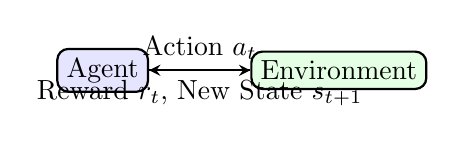
\begin{tikzpicture}[node distance=3cm, auto, >=stealth]
    \node[draw, rounded corners, thick, fill=blue!10] (agent) {Agent};
    \node[draw, rounded corners, thick, fill=green!10, right of=agent] (env) {Environment};

    \draw[->, thick] (agent) -- node[above]{Action $a_t$} (env);
    \draw[->, thick] (env) -- node[below]{Reward $r_t$, New State $s_{t+1}$} (agent);
\end{tikzpicture}
\caption{RL agent-environment interaction loop}
\end{figure}

% -----------------------------------------------------------
\subsection{Markov Decision Process (MDP)}

An MDP is defined by:
\begin{itemize}
    \item States $S$
    \item Actions $A$
    \item Transition probabilities $P(s'|s,a)$
    \item Reward function $R(s,a)$
    \item Discount factor $\gamma \in [0,1]$
\end{itemize}

The goal: maximize cumulative discounted reward
\[
G_t = \sum_{k=0}^{\infty} \gamma^k r_{t+k}
\]

% -----------------------------------------------------------
\subsection{Value Functions and Q-Learning}

State-value function:
\[
V^\pi(s) = \mathbb{E}_\pi[G_t \mid s_t = s]
\]

Action-value (Q-function):
\[
Q^\pi(s,a) = \mathbb{E}_\pi[G_t \mid s_t = s, a_t = a]
\]

Optimal policy:
\[
\pi^*(s) = \arg\max_a Q^*(s,a)
\]

Q-learning update:
\[
Q(s_t,a_t) \leftarrow Q(s_t,a_t) + \alpha \bigl(r_t + \gamma \max_{a'} Q(s_{t+1},a') - Q(s_t,a_t)\bigr)
\]

% -----------------------------------------------------------
\subsection{Example: Robot, Banana Peel, Apple}

\begin{itemize}
    \item $R$: Robot, $B$: Banana peel, $A$: Apple
    \item Rewards: $R_A = 100$, $R_\text{alive} = 40$, $R_B = -100$
    \item Agent chooses actions (left/right) to maximize cumulative reward
\end{itemize}

% -----------------------------------------------------------
\subsection{Exploration vs Exploitation}

\begin{itemize}
    \item \textbf{Exploitation:} Choose best-known action
    \item \textbf{Exploration:} Try new actions to find better outcomes
\end{itemize}

$\varepsilon$-Greedy policy:
\begin{itemize}
    \item With probability $\varepsilon$, select a random action
    \item With probability $1-\varepsilon$, select $a_t = \arg\max_a Q_t(a)$
\end{itemize}

\textbf{Optimistic Initial Values (OIV):} Start $Q_1(a)$ high to encourage exploration.

% -----------------------------------------------------------
\subsection{K-Armed Bandit Problem}

\begin{itemize}
    \item $k$ slot machines with unknown reward distributions
    \item Goal: maximize total reward over time
    \item Update rule:
    \[
    Q_{t+1}(a) = Q_t(a) + \frac{1}{N_t(a)} (R_t - Q_t(a))
    \]
    \item Balance exploration and exploitation
\end{itemize}

\subsubsection{Upper Confidence Bound (UCB)}

Action selection:
\[
a_t = \arg\max_a \left[ Q_t(a) + c \sqrt{\frac{\ln t}{N_t(a)}} \right]
\]

\subsubsection{Gradient Bandits}

Use preference $H_t(a)$ and softmax policy:
\[
\pi_t(a) = \frac{e^{H_t(a)}}{\sum_b e^{H_t(b)}}
\]
Update $H_t(a)$ in the direction of higher reward.